% File tacl2018v2.tex
% Sep 20, 2018

% The English content of this file was modified from various *ACL instructions
% by Lillian Lee and Kristina Toutanova
%
% LaTeXery is mostly all adapted from acl2018.sty.

\documentclass[11pt,a4paper]{article}
\usepackage{times,latexsym}
\usepackage{url}
\usepackage[T1]{fontenc}

%% Package options:
%% Short version: "hyperref" and "submission" are the defaults.
%% More verbose version:
%% Most compact command to produce a submission version with hyperref enabled
%%    \usepackage[]{tacl2018v2}
%% Most compact command to produce a "camera-ready" version
%%    \usepackage[acceptedWithA]{tacl2018v2}
%% Most compact command to produce a double-spaced copy-editor's version
%%    \usepackage[acceptedWithA,copyedit]{tacl2018v2}
%
%% If you need to disable hyperref in any of the above settings (see Section
%% "LaTeX files") in the TACL instructions), add ",nohyperref" in the square
%% brackets. (The comma is a delimiter in case there are multiple options specified.)

\usepackage[]{tacl2018v2}

%%%% Material in this block is specific to generating TACL instructions
\usepackage{xspace,mfirstuc,tabulary}
\newcommand{\dateOfLastUpdate}{Sept. 20, 2018}
\newcommand{\styleFileVersion}{tacl2018v2}

\newcommand{\ex}[1]{{\sf #1}}

\newif\iftaclinstructions
\taclinstructionsfalse % AUTHORS: do NOT set this to true
\iftaclinstructions
\renewcommand{\confidential}{}
\renewcommand{\anonsubtext}{(No author info supplied here, for consistency with
TACL-submission anonymization requirements)}
\newcommand{\instr}
\fi

%
\iftaclpubformat % this "if" is set by the choice of options
\newcommand{\taclpaper}{final version\xspace}
\newcommand{\taclpapers}{final versions\xspace}
\newcommand{\Taclpaper}{Final version\xspace}
\newcommand{\Taclpapers}{Final versions\xspace}
\newcommand{\TaclPapers}{Final Versions\xspace}
\else
\newcommand{\taclpaper}{submission\xspace}
\newcommand{\taclpapers}{{\taclpaper}s\xspace}
\newcommand{\Taclpaper}{Submission\xspace}
\newcommand{\Taclpapers}{{\Taclpaper}s\xspace}
\newcommand{\TaclPapers}{Submissions\xspace}
\fi

%%%% End TACL-instructions-specific macro block
%%%%


%%%% Start personalised macro block
\usepackage{amssymb}
\usepackage{graphicx}
\usepackage{tabularx}

\newcommand{\mvec}[1]{$\mathbf{#1}$\xspace}
\newcommand{\name}[1]{\textsl{#1}\xspace}
\renewcommand{\vec}[1]{\mathbf{#1}\xspace}

\newcommand{\cs}[1]{\begin{color}{blue}CS: #1\end{color}\xspace}
\newcommand{\tbd}[1]{\begin{color}{red}TBD: #1\end{color}\xspace}
%%%% End personalised macro block

\title{}

% Author information does not appear in the pdf unless the "acceptedWithA" option is given
% See tacl2018v2.sty for other ways to format author information
\author{
 Template Affiliation/Address Line 1 \\
 Template Affiliation/Address Line 2 \\
 Template Affiliation/Address Line 2 \\
  {\sf template.email@sampledomain.com} \\
}

\date{}

\begin{document}
\maketitle
\begin{abstract}

\begin{itemize}
	\item We address the task of human object naming: given an object that is depicted in an image, produce the name for it. 
	\item While people, when being asked to name an object, tend to agree on a specific name in many cases, there is also variation (REF). The choice of a name for an individual object can thus be considered to underlie some probability distribution over possible names, representing naming preferences. 
	%Individual objects can thus be associated with naming preferences instead of a unique name. 
	\cs{How could we examine in how far/under which conditions the difference in rankings between two objects is not by chance? randomised test?}
	\item Variation can be effected by several factors, such as the appearance of the object itself, or its situated context (both have been studied in psychological research, REF). 
	\item Our goal is to understand the factors which play a role in preferring one name over valid name alternatives for individual objects. 
	\item We formulate the task of object naming as the prediction of  object name preferences, and present XXX model. 
	\item We examine the factors: 
	\item Our results show that XXX.
	
\end{itemize}
 
\end{abstract}

\section{Introduction}
\label{sec:introduction}

\cs{How to formulate it? As label distribution learning or as preference learning? (See related work)}

\section{Related Work}
\label{sec:related}

\subsection{Referring Expression Comprehension/Generation}
\cs{relevant for choosing comparison models / models to build upon; urls see tex source}\\
Current SOTA on RefCOCO+/g, in descending order of accuracy:\\

\paragraph{Transformer}
\noindent
Su et al. (2019): VL-BERT: PRE-TRAINING OF GENERIC VISUAL-LINGUISTIC REPRESENTATIONS\\
\cs{Work in progress, results only on RefCOCO+: } compared to VilBERT (below), no seprate vis and lang transformers in early parts of the model, but attention over both modalities from early on; no pre-training on visual-language relation prediction. FRCNN parameters updated during training. \url{arxiv.org/pdf/1908.08530.pdf}\\

\paragraph{Gated Graph ConvNet}
\noindent
Yang et al. (CVPR 2019): Cross-Modal Relationship Inference for Grounding Referring Expressions\\
%\url{openaccess.thecvf.com/content_CVPR_2019/papers/Yang_Cross-Modal_Relationship_Inference_for_Grounding_Referring_Expressions_CVPR_2019_paper.pdf}\\

\paragraph{Transformers}
\noindent
Lu et al. (NIPS 2019): ViLBERT: Pretraining Task-Agnostic Visio-linguistic Representations for Vision-and-Language Tasks\\
In "modelling task", VilBERT is pre-trained to minimise the KL divergence between its input---masked softmax prediction obtained from FRCNN---and its output---reconstruction of the input. In the "multi-modal alignment" task, the model is pre-trained to determine whether image and text match, based on a joint hidden representation (element-wise product of hidden vectors).\\
 \url{arxiv.org/pdf/1908.02265.pdf}\\
 Follow-up: 12-in-1 [...] (work in progress):\\
\url{arxiv.org/pdf/1912.02315.pdf}\\

\noindent
Liu et al. (CVPR 2019): Improving Referring Expression Grounding
with Cross-modal Attention-guided Erasing\\
%\url{openaccess.thecvf.com/content_CVPR_2019/papers/Liu_Improving_Referring_Expression_Grounding_With_Cross-Modal_Attention-Guided_Erasing_CVPR_2019_paper.pdf}\\

\noindent
Wang et al. (CVPR 2019): Neighbourhood Watch: Referring Expression Comprehension via
Language-guided Graph Attention Networks\\
%\url{openaccess.thecvf.com/content_CVPR_2019/papers/Wang_Neighbourhood_Watch_Referring_Expression_Comprehension_via_Language-Guided_Graph_Attention_Networks_CVPR_2019_paper.pdf}\\

\subsection{Object Recognition}
\newcite{kang2019decoupling}: long-tailed recognition

\subsection{Multi-Label Learning / Multi-Target Learning}
Sorower (2010)

\noindent
Xu et al. (2019)\\
\url{ieeexplore.ieee.org/abstract/document/8892612}\\

\noindent
ML:\\
\textbf{Label distribution learning (DLD; Geng, 2016)}\\ \url{ieeexplore.ieee.org/stamp/stamp.jsp?tp=&arnumber=7439855}\\
Single-label approach in object recognition, where the object is assigned the most frequently assigned label, underlies the wrong assumption that the relative frequency of the label expresses the \textit{probability} of it being the correct label. Instead, all annotations may be correct, such that the relative frequency of a label~$l$ in fact expresses the \textit{degree of preference} of~$l$ over the other labels.   \\ 

\noindent
NLP:\\
Zhou et al. (2016) Emotion Distribution Learning from Texts\\
\url{www.aclweb.org/anthology/D16-1061.pdf}\\

\noindent
Visual Emotion Classification: \\
%LDL: related to object naming in that different names can be true for an object (intensity of emotion == degree of preference for name), and naming underlies diverse social and cultural background \\
Yang et al. (2017): tasks of emotion classification and distribution prediction  \url{www.ijcai.org/Proceedings/2017/0456.pdf}\\
-- softmax for classification, and additionally KL loss\\

\noindent
\textbf{Preference Learning}\\
-- Graded Multilabel Classification: The Ordinal Case\\
\url{www.kde.cs.uni-kassel.de/wp-content/uploads/conf/lwa10/papers/kdml18.pdf}   \\
\noindent
-- Label Ranking by Learning Pairwise Preferences\\
\url{www.ke.tu-darmstadt.de/~juffi/publications/aij-08.pdf}\\

\noindent
Object recognition: \\
-- Gao et al. (2017)\\ \url{ieeexplore.ieee.org/stamp/stamp.jsp?tp=&arnumber=7890384}\\

\noindent
NLP:\\
-- Fuernkranz et al. (2008) \url{link.springer.com/content/pdf/10.1007/s10994-008-5064-8.pdf}\\
-- (Patent)
\url{patents.google.com/patent/US20190251446A1/en}\\



\section{MODELNAME for Human Object Naming}
\label{sec:method}

\subsection{Architecture}
\label{ssec:model_architecture}
\tbd{START}
\cs{NOTE START}
A graph-based model (as shortly talked about in the last object naming meeting) would make sense if the task was refexp generation/interpretation, where there exists a mutual dependence between the objects and their respective refexps, and the refexp itself encodes relational information between the objects (e.g., \textsl{Y beside X})---the nodes would be the different objects, and the edges would be used to exchange information which effects the determination of a \textit{unique} linguistic reference (generation) for each of them.\\
So, I am favouring a transformer-based NN architecture, without a graph-structure, with self-attention (target object and the input information), and cross-attention (between different objects).
\cs{NOTE END}

\textbf{\cs{I'll add content to the actual architecture tomorrow. But feel free to comment on everything that is here by now / add things to the document.}}

\paragraph{Features (/Input)}
Let $\mathcal{X} = \mathbb{R}^q$ denote the input space, and $\mathcal{N} = \{n_1, n2, \dots, n_N\}$ denote the complete set of names. 
Given a training set $\mathcal{M} = \{({ x_1},R_1), ({ x_2},R_2),\dots,({ x_n},R_n)\}$ of tuples target object representations and name responses. \\
Input ${x_i}$ for target object $o_i$ comprises one or more of the following information:
\begin{description}
	\item[Visual:] $\mathbf{v_i}$, $\mathbf{v_1}, \dots, \mathbf{v_k}$; $\mathbf{s_i}$, $\mathbf{s_1}, \dots, \mathbf{s_k}$; $\mathbf{v_g}$
	\begin{itemize}
		\item Target object representation:\\
		-- image features $\mathbf{v_i}$ of bounding box $\mathbf{b_i}$ of $o_i$ \cs{see below for image features}\\
		-- spatial location features $\mathbf{s_i}$: 5-d vector with normalised top left and bottom right location and relative size (standard features for grounding tasks, such as refexp comprehension, visual semantic role labeling)
		\item Context representation:\\
		-- image features $\mathbf{v_1}, \dots, \mathbf{v_k}$ of other objects $o_1, \dots, o_k; i \notin \{1, \dots, k\}$\\
		option: only objects whose boxes $\mathbf{b_1}, \dots, \mathbf{b_k}$ overlap with box $\mathbf{b_i}$ (e.g., food domain); or no restriction on objects (e.g., racket in image (a), Table~\ref{tab:player_statue})\\
		-- spatial location features of other objects $\mathbf{s_1}, \dots, \mathbf{s_k}$\\
		-- AND/OR: "global" image features, encoding whole image $\mathbf{v_g}$
		%\item Target + context representation:\\
		%-- spatial location features: (standard features for grounding tasks, such as refexp comprehension, visual semantic role labeling)
	\end{itemize}
	\item[Language:] None, $\vec{l_i}$, $\vec{l_1}, \dots, \vec{l_k}$; $\vec{l^g_i}$,  $\vec{l^g_1}, \dots, \vec{l^g_k}$
	\begin{itemize}
		\item Target object:\\
		(A) for ranking loss objective:\\
		-- embedding(s) $\vec{l_i}$ of candidate name(s)\\
		-- length of name, in letters\\
		(B) for KL divergence objective:\\
		-- None \\
		-- embedding $\vec{l^g_i}$ of VG name \cs{does this make sense!?}
		\item Context objs. \mbox{$o_1, \dots, o_k; i \notin \{1, \dots, k\}$}\\
		-- None \\
		-- embeddings $\vec{l_1}, \dots, \vec{l_k}$ of MN names\\
		-- embeddings $\vec{l^g_1}, \dots, \vec{l^g_k}$ of VG names \cs{does this make sense!?}\\
	\end{itemize}
\end{description}

\paragraph{Data}
Image features $\mathbf{v}$
\begin{itemize}
	\item Faster-RCNN, pre-trained on ImageNet?
	\item Faster-RCNN, pre-trained on VG? (Bottom-Up)
	\item ResNet-101? (lower layers, not before softmax output (!))
\end{itemize}
\tbd{END}

\noindent
\tbd{START}
\subsection{Training}
\label{ssec:model_training}
\begin{itemize}
	\item Pre-train on, e.g., VG
	\item Fine-tune on ManyNames 
	%\item [Apply GAN -- generator does not receive visual input.]
	\item View it as Label Distribution Learning, or more generally Preference Order Learning? In the former, the degree of preference (i.e., the actual value) is important, in the latter it's only the ranking of labels according to preference. 
\end{itemize}
\textbf{Ranking loss (max-margin loss)} or \textbf{Label-Ranking Loss} (multiple labels per instance; takes into account the ranking of all labels\footnote{\url{scikit-learn.org/stable/modules/model_evaluation.html}})\\
\cs{Arguments for ranking loss: 
\begin{itemize}
	\item during training, the target name for an instance could be sampled according to its response distribution, thus implicitly learning the distribution / ranking; also, we cannot assume the response distribution to be correct, but it is rather an estimate of the true distribution
	\item we can use the same model for pre-training and fine-tuning: sample highly unlikely negative names from vocabulary
	\item \textbf{for fine-tuning on MN, for the "difficult" cases, we could get negative names for free from the verification data (low adequacy score or wrong cluster)}
	\item using a sigmoid or tanh activation function which feeds the loss function, we could set the margin such that it mirrors the order of preference (higher margin for highly preferred names, lower for less preferred names (is that numerically stable?!))
	\item experimentally successful
	\item fits the view on naming is a matter of preference over multiple names
\end{itemize}
}

\textbf{Normalized Discounted Cumulative Gain}\\
Ranking metric, where only gt labels are considered for computing the loss\footnote{\url{https://scikit-learn.org/stable/modules/model_evaluation.html}}.\\

\textbf{Kullback-Leibler divergence loss (KL loss)}\\

\subsection{Testing}
\begin{itemize}
	\item For ranking objective: compute score for each word in the vocabulary, produce a probability distribution by applying softmax / normalising
	\item For KL divergence objective using a softmax output layer: take directly  output
\end{itemize}
\tbd{END}

\section{Experiments}
\label{sec:experiments}

\paragraph{Questions}
\begin{itemize}
	\item How do we learn these  name preferences?\\
	 (Model itself, TBD) How do we incorporate rankings of names into the training procedure? Is the ManyNames data big enough to do that?
	\item Do contextual features (which ones?) influence the ranking? (refs: \citealp{murphy1989categorizing})\\
	Can we formulate a ``multimodal analogy task''?
	\begin{itemize}
		\item Are specific context objects determinative of the name (e.g., skies+person -> skier; salad;)?
		\item Is there a dependence on the event/situation and the object name on the model effectiveness?  (e.g., TBD)\\
		additional task on action recognition (see also \newcite{Rosch1978} and "basic-level" objects: the most general classes which have common motor sequences)
	\end{itemize}
	\item Appearance of object: prototypicality? lexical factors (familiarity, length)?
\end{itemize}

\paragraph{Minor Questions (for analysis)}
\begin{itemize}
	\item For which domains does context play a more important role?
	\item When entry-level name diverges from object classes' entry-level name (e.g., duck vs. bird), is that due to
	- context?
	- prototypicality (i.e., object itself)?
\end{itemize}

\subsection{Tasks}
\label{ssec:exp_task}

\begin{table*}[t]
\begin{tabularx}{\textwidth}{XXX}
\multicolumn{1}{c}{\textbf{parrot}} 
& \multicolumn{1}{c}{\textbf{bird?}} 
&\multicolumn{1}{c}{\textbf{bird}} \\
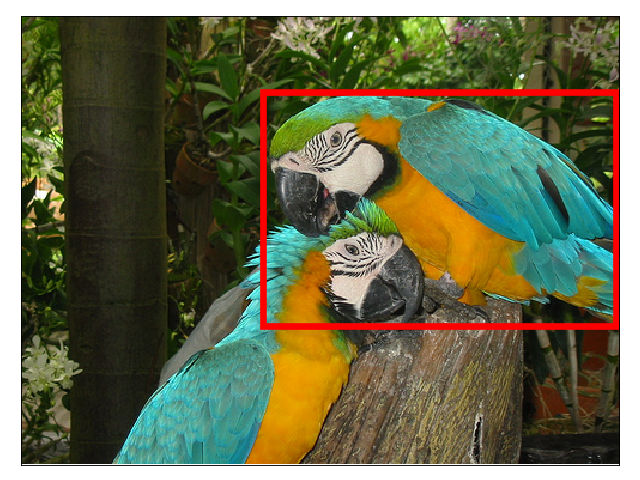
\includegraphics[width=0.6\columnwidth]{images/2371393_739660_seed_ambiguous.png}
& 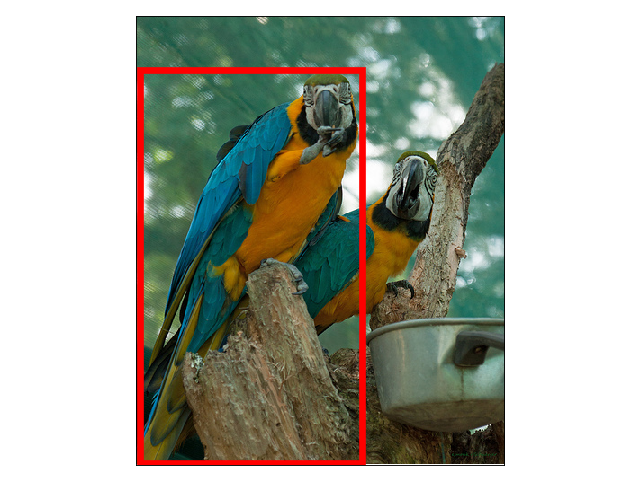
\includegraphics[width=0.6\columnwidth]{images/2356387_820983_singleton_obj.png}
& 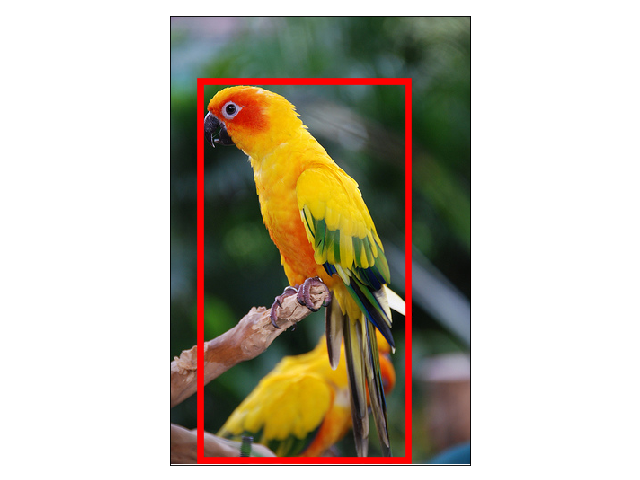
\includegraphics[width=0.6\columnwidth]{images/2341058_944671_singleton_obj.png}
\\
(a) 'parrot': 18, 'bird': 12
% {'bird': {'cluster': ('bird', 'parrot'), 'adequacy': 1.0, 'inadequacy_type': None, 'cluster_id': 0, 'cluster_weight': 1.0}, 'parrot': {'cluster': ('bird', 'parrot'), 'adequacy': 1.0, 'inadequacy_type': None, 'cluster_id': 0, 'cluster_weight': 1.0}}
& (b) 'bird': 22, 'parrot': 14
%{'parrot': {'cluster': ('bird', 'parrot'), 'adequacy': 1.0, 'inadequacy\_type': None, 'cluster\_id': 0, 'cluster\_weight': 1.0}, 'bird': {'cluster': ('bird', 'parrot'), 'adequacy': 1.0, 'inadequacy\_type': None, 'cluster\_id': 0, 'cluster\_weight': 1.0}}
& (c) 'bird': 27, 'parrot': 9	
%{'parrot': {'cluster': ('bird', 'parrot'), 'adequacy': 1.0, 'inadequacy\_type': None, 'cluster\_id': 0, 'cluster\_weight': 1.0}, 'bird': {'cluster': ('bird', 'parrot'), 'adequacy': 1.0, 'inadequacy\_type': None, 'cluster\_id': 0, 'cluster\_weight': 1.0}}
\\
%%%
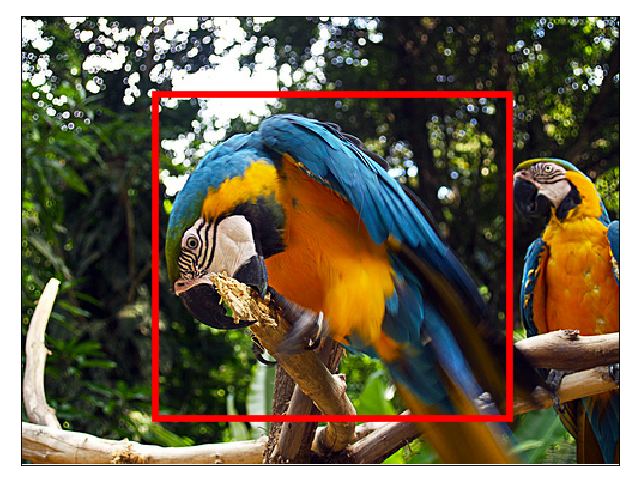
\includegraphics[width=0.6\columnwidth]{images/2349587_2162340_seed_ambiguous.png}
& 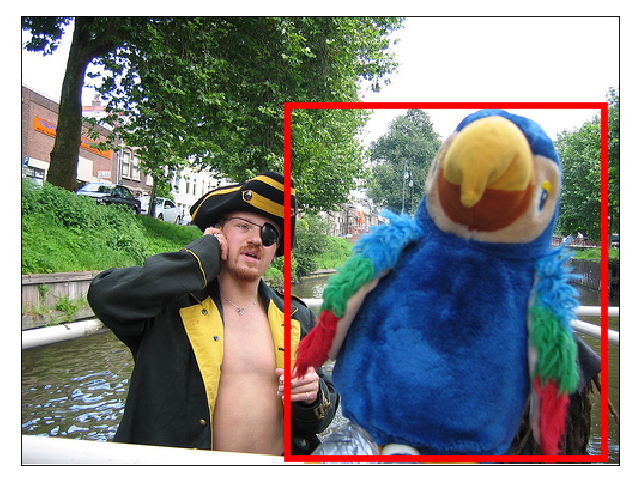
\includegraphics[width=0.6\columnwidth]{images/2332379_2755215_supercat_unique.png}
& 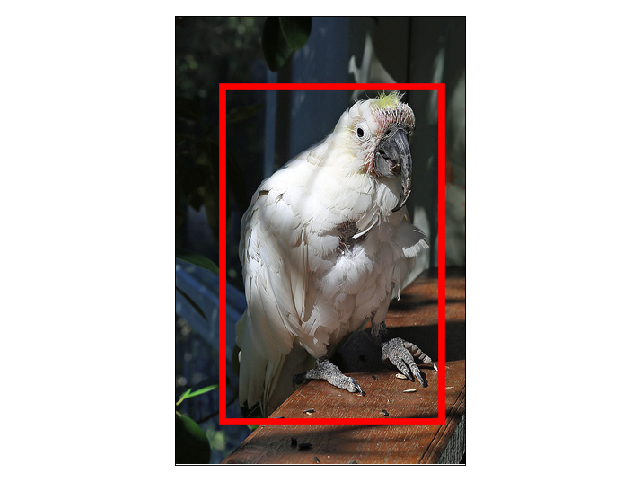
\includegraphics[width=0.6\columnwidth]{images/2348089_2328048_seed_ambiguous.png}
\\
(d) 'parrot': 20, 'bird': 14
%	{'parrot': {'cluster': ('bird', 'parrot'), 'adequacy': 1.0, 'inadequacy\_type': None, 'cluster\_id': 0, 'cluster\_weight': 1.0}, 'bird': {'cluster': ('bird', 'parrot'), 'adequacy': 1.0, 'inadequacy\_type': None, 'cluster\_id': 0, 'cluster\_weight': 1.0}}
& (e) 'bird': 16, 'parrot': 7, 'toy': 4, 'stuffed animal': 3, 'plushier': 2
%{'toy': {'cluster': ('bird', 'parrot', 'plushier', 'stuffed animal', 'toy'), 'adequacy': 1.0, 'inadequacy\_type': None, 'cluster\_id': 0, 'cluster\_weight': 1.0}, 'bird': {'cluster': ('bird', 'parrot', 'plushier', 'stuffed animal', 'toy'), 'adequacy': 1.0, 'inadequacy\_type': None, 'cluster\_id': 0, 'cluster\_weight': 1.0}, 'stuffed animal': {'cluster': ('bird', 'parrot', 'plushier', 'stuffed animal', 'toy'), 'adequacy': 1.0, 'inadequacy\_type': None, 'cluster\_id': 0, 'cluster\_weight': 1.0}, 'plushier': {'cluster': ('bird', 'parrot', 'plushier', 'stuffed animal', 'toy'), 'adequacy': 0.5, 'inadequacy\_type': 'linguistic', 'cluster\_id': 0, 'cluster\_weight': 1.0}, 'parrot': {'cluster': ('bird', 'parrot', 'plushier', 'stuffed animal', 'toy'), 'adequacy': 1.0, 'inadequacy\_type': None, 'cluster\_id': 0, 'cluster\_weight': 1.0}}
& (f) 'bird': 30, 'parrot': 5
%{'parrot': {'cluster': ('bird', 'parrot'), 'adequacy': 1.0, 'inadequacy\_type': None, 'cluster\_id': 0, 'cluster\_weight': 1.0}, 'bird': {'cluster': ('bird', 'parrot'), 'adequacy': 1.0, 'inadequacy\_type': None, 'cluster\_id': 0, 'cluster\_weight': 1.0}}
\end{tabularx}
\caption{\label{tab:parrot} Parrot vs. bird}
\end{table*}

\begin{table*}[t]
	\begin{tabularx}{\textwidth}{XXX}
		\multicolumn{1}{c}{\textbf{woman / tennis player}} 
		& \multicolumn{1}{c}{\textbf{horse / statue}} 
		&\multicolumn{1}{c}{\textbf{statue / bird}} \\
		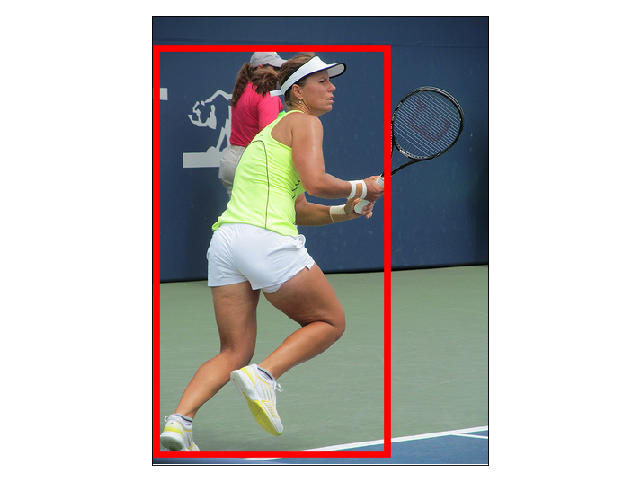
\includegraphics[width=0.6\columnwidth]{images/2384231_692300_singleton_obj.png}
		& 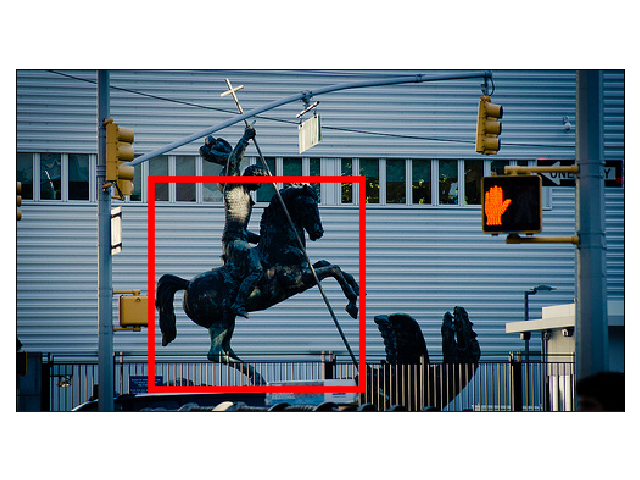
\includegraphics[width=0.6\columnwidth]{images/2374110_2599202_singleton_obj.png}
		& 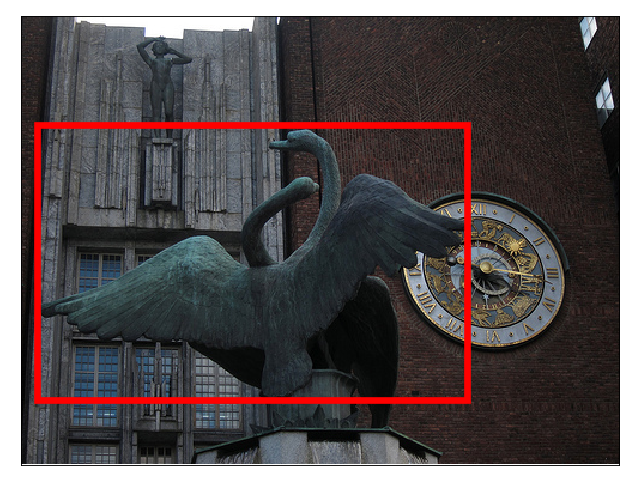
\includegraphics[width=0.6\columnwidth]{images/2387975_676194_seed_ambiguous.png}
		\\
		(a) 'woman': 17, 'tennis player': 11, 'athlete': 3, 'player': 3, 'person': 2
		& 'horse': 30, 'statue': 5
		& 'statue': 19, 'bird': 8
		\\
		%%%
		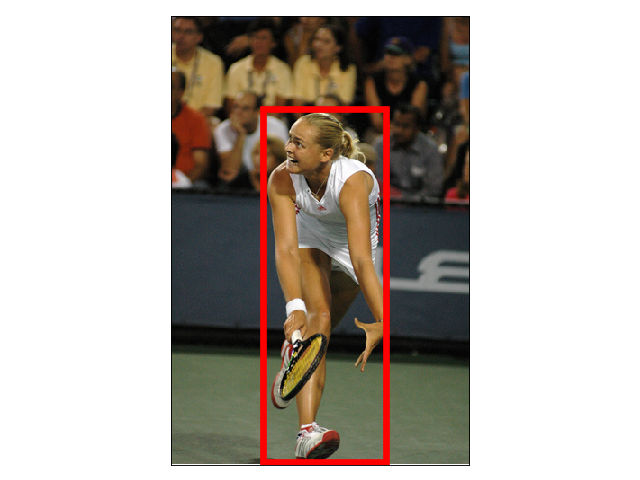
\includegraphics[width=0.6\columnwidth]{images/2321096_1048648_singleton_obj.png}
		& 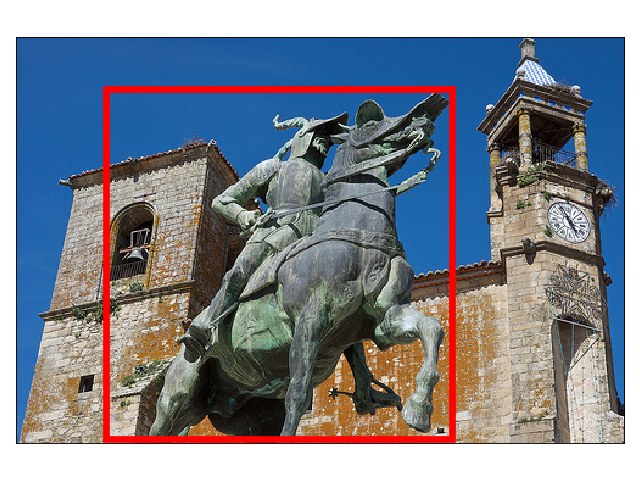
\includegraphics[width=0.6\columnwidth]{images/2362660_2481248_supercat_unique.png}
		& 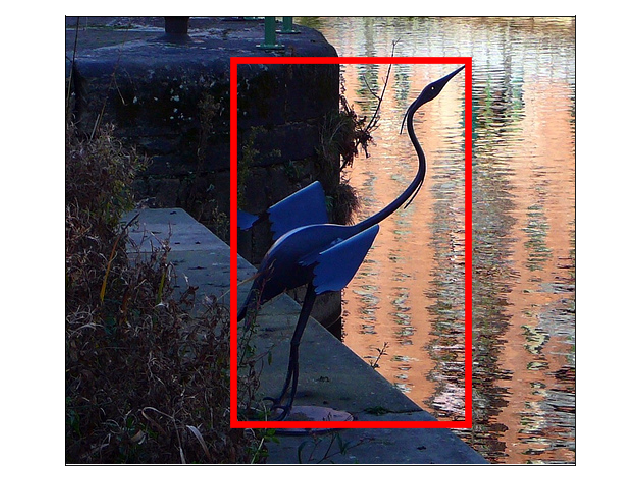
\includegraphics[width=0.6\columnwidth]{images/2332099_3492153_singleton_obj.png}\\
		'tennis player': 14, 'woman': 6, 'player': 4, 'shoe': 3, 't-shirt': 2
		& 'statue': 33
		& 'bird': 26, 'swan': 2, 'statue': 2
		\\
	
	\end{tabularx}
	\caption{\label{tab:player_statue} }
\end{table*}

\tbd{START (minor)}
\cs{Focus on Task 1("full task"), subtasks can be addressed later.}\\
Let $\mathcal{X} = \mathbb{R}^q$ denote the input space, and $\mathcal{N} = \{n_1, n2, \dots, n_N\}$ denote the complete set of names. 
Given a training set $\mathcal{M} = \{({\bf x_1},R_1), ({\bf x_2},R_2),\dots,({\bf x_n},R_n)\}$ of tuples of objects and name responses. 
\begin{enumerate}
	\item As a first step towards Task 2 below, we address the task of agreement prediction \cs{better name for this needed}, i.e.,~$R_i \in \mathbb{N}$ is simply the cardinality of the response set (types) of instance~$\mathbf{x}_i$.\\
	$\Rightarrow$ Factor out the linguistic factors involved in the choice of a name, and analyse the effectiveness of the model on the level of instances/classes/domains, and the influence of the factors under examination (input features). Especially interesting: cases such as object~(e) (visual appearance of instance; Table~\ref{tab:parrot}), and object~(a) (domain; Table~\ref{tab:player_statue}). \\
	$\Rightarrow$ Compare model effectiveness on this task with that on the full task, and analyse with respect to input factors and instances/classes/domains.
	\item Predicting  name preferences (full task)	
	\cs{How do we evaluate this? (see also training losses above) Suggestions:}
	\begin{enumerate}
		\item \textbf{Probability distribution}\\
		Interpret $R_i$ as name response distribution for instance $\mathbf{x}_i$, i.e., the task is to learn a conditional probability mass function $p(y|\mathbf{x};\theta)$ from $\mathcal{M}$, where ${\bf x} \in \mathcal{X}$, $y \in \mathcal{N}$.  $\theta$ are the parameters generating the a distribution that approximates $R_i$ for an instance $\mathbf{x}_i$.
		\item Alternatives: \\
		-- \textbf{Preference Learning}\\
		Interpret $R_i$ as a ranking of name responses, i.e., the actual scores are not considered. 
		E.g.,~woman $>$ tennis player $>$ athlete/player $>$ person (image (a) in Table~\ref{tab:player_statue}) \cs{??possible problem: (near-)ties are not considered}\\
		-- Average reciprocal rank?\\
		-- ... ?
	\end{enumerate}
	\item Subtask 1: Entry-level only\\
	Generation: Given an object, predict its top-responded name (e.g.,~\name{parrot} for images on the left, Table~\ref{tab:parrot}).
	\item Subtask 2: Determine representative of a given name: Which of these two objects is more of an X?\\	
	Interpretation: Given two objects and a name, (o1,o2,nj), determine which object is more likely to be meant. For instance, for (img(a), img(f), \name{parrot}), it would be img(a), and img(f) for nj=\name{bird} (Table~\ref{tab:parrot}).\\
	Related to: prototypicality\\
	-- Task setup:
	Each item consists of two objects and a name nj, (o1,o2,nj), with nj being valid for both, o1 and o2, but the entry-level name for only one of the two objects. 
	%-- Evaluation for Task (i): Is the predicted object’s entry-level name == nj?
	%
	\item \cs{NEW Subtask 3: "Taboo"-game: Given some object names $o_1, \dots, o_k$, predict another alternative name $o_j$ (Assuming $o_1, \dots, o_k$ is in descending order of preference, target could be sampled such that $1<j<k$).  Extra tricky subset: $k=1$}
\end{enumerate}
\tbd{END (minor)}


\subsection{Experimental Setup}
\label{ssec:exp_setup}

\subsection{Results}
\label{ssec:exp_results}

\section{Conclusions}
\label{sec:conclusions}

\section{Notes}
\begin{itemize}
	\item Hypothesis: Naming variation is higher in domains for which humans naturally have "close-to-expert" knowledge, e.g., food, people.\\
	\newcite{tanaka1991object}: \textit{``The main findings were that in the domain of expertise (a) subordinate-level categories were as differentiated as the basic-level categories, (b) subordinate-level names were used as frequently as basic-level names for identifying objects, and(c) subordinate-level categorizations were as fast as basic-level categorizations. [...]\\
		one might hypothesize a downward shift in the basic level or the creation of a
		second more specific basic level in a classification hierarchy as a function
		of expertise. ''}
\end{itemize}

\section{Appendices} 
\label{sec:appendix}
Appendices, if any, directly follow the text and the
references.  Recall that {\em appendices count
towards the page limit.}


\bibliography{naming}
\bibliographystyle{acl_natbib}

\end{document}


